% Some commands used in this file
\newcommand{\package}{\emph}

\chapter{Introduction}
\section{Background}
The omnidirectionality of loudspeakers is not always something to aspire to but rather something that should be suppressed. This can be done by using nonlinear characteristics of air in a phenomenon known as "sound from ultrasound". With this principle, one can create a highly directional steerable audio beam. 

Until now, many studies have been conducted in the field of "sound from ultrasound" and the theory of its inner workings has been mostly understood. Nevertheless, no commercially available loudspeaker can do this. Due to this, we decided to use this theory gained from years of research and combine it with our ideas to create a fully functional device, the Audio-Beamformer. 

There are many potential use cases for such loudspeakers. Be it as a possibility to direct the sound of a phone call to only the person sitting right in front of a computer and mitigating the need to wear headphones or the possibility to sit with foreign friends on the same couch and watch a movie in different languages. 
\section{Scope}
Around the task given, which can be seen in Appendix \ref{definition_of_task}, we defined our own goals we wanted to reach in the scope of this thesis. 
Our first goal was to dive deep into the theory of how to generate a highly directional and steerable audio beam and get a good overview of the different technologies and ideas implemented. 
The second goal was to design the product. For this, we set ourselves a bunch of additional goals. We set the goal to create not only a working "sound from ultrasound" loudspeaker but also make it highly professional and easy to use. A product which is perfect for demonstration purposes.
\newpage

\section{Approach}
To achieve our goal, we started by researching different theories on creating directional sound.
We decided right from the start that the "sound from ultrasound" Principe was the way to go, mainly because of the higher directivity.
After that, we looked for hardware that was already built to get an idea and a feeling for this kind of loudspeaker. However, as there is no commercially available product, we had to develop the hardware ourselves.
For this, we made multiple iterations of prototypes, starting with a basic buildup on a breadboard, then soldering everything to a stripboard. After that, we designed and ordered a prototype \acrshort{pcb} and, in the end, redesigned the prototype once again and ordered the final \acrshort{pcb}.  
To test everything and quantify the results we got, we measured everything extensively with a dedicated ultrasonic microphone and human expertise tests.

\begin{figure}[h!]
	\centering
	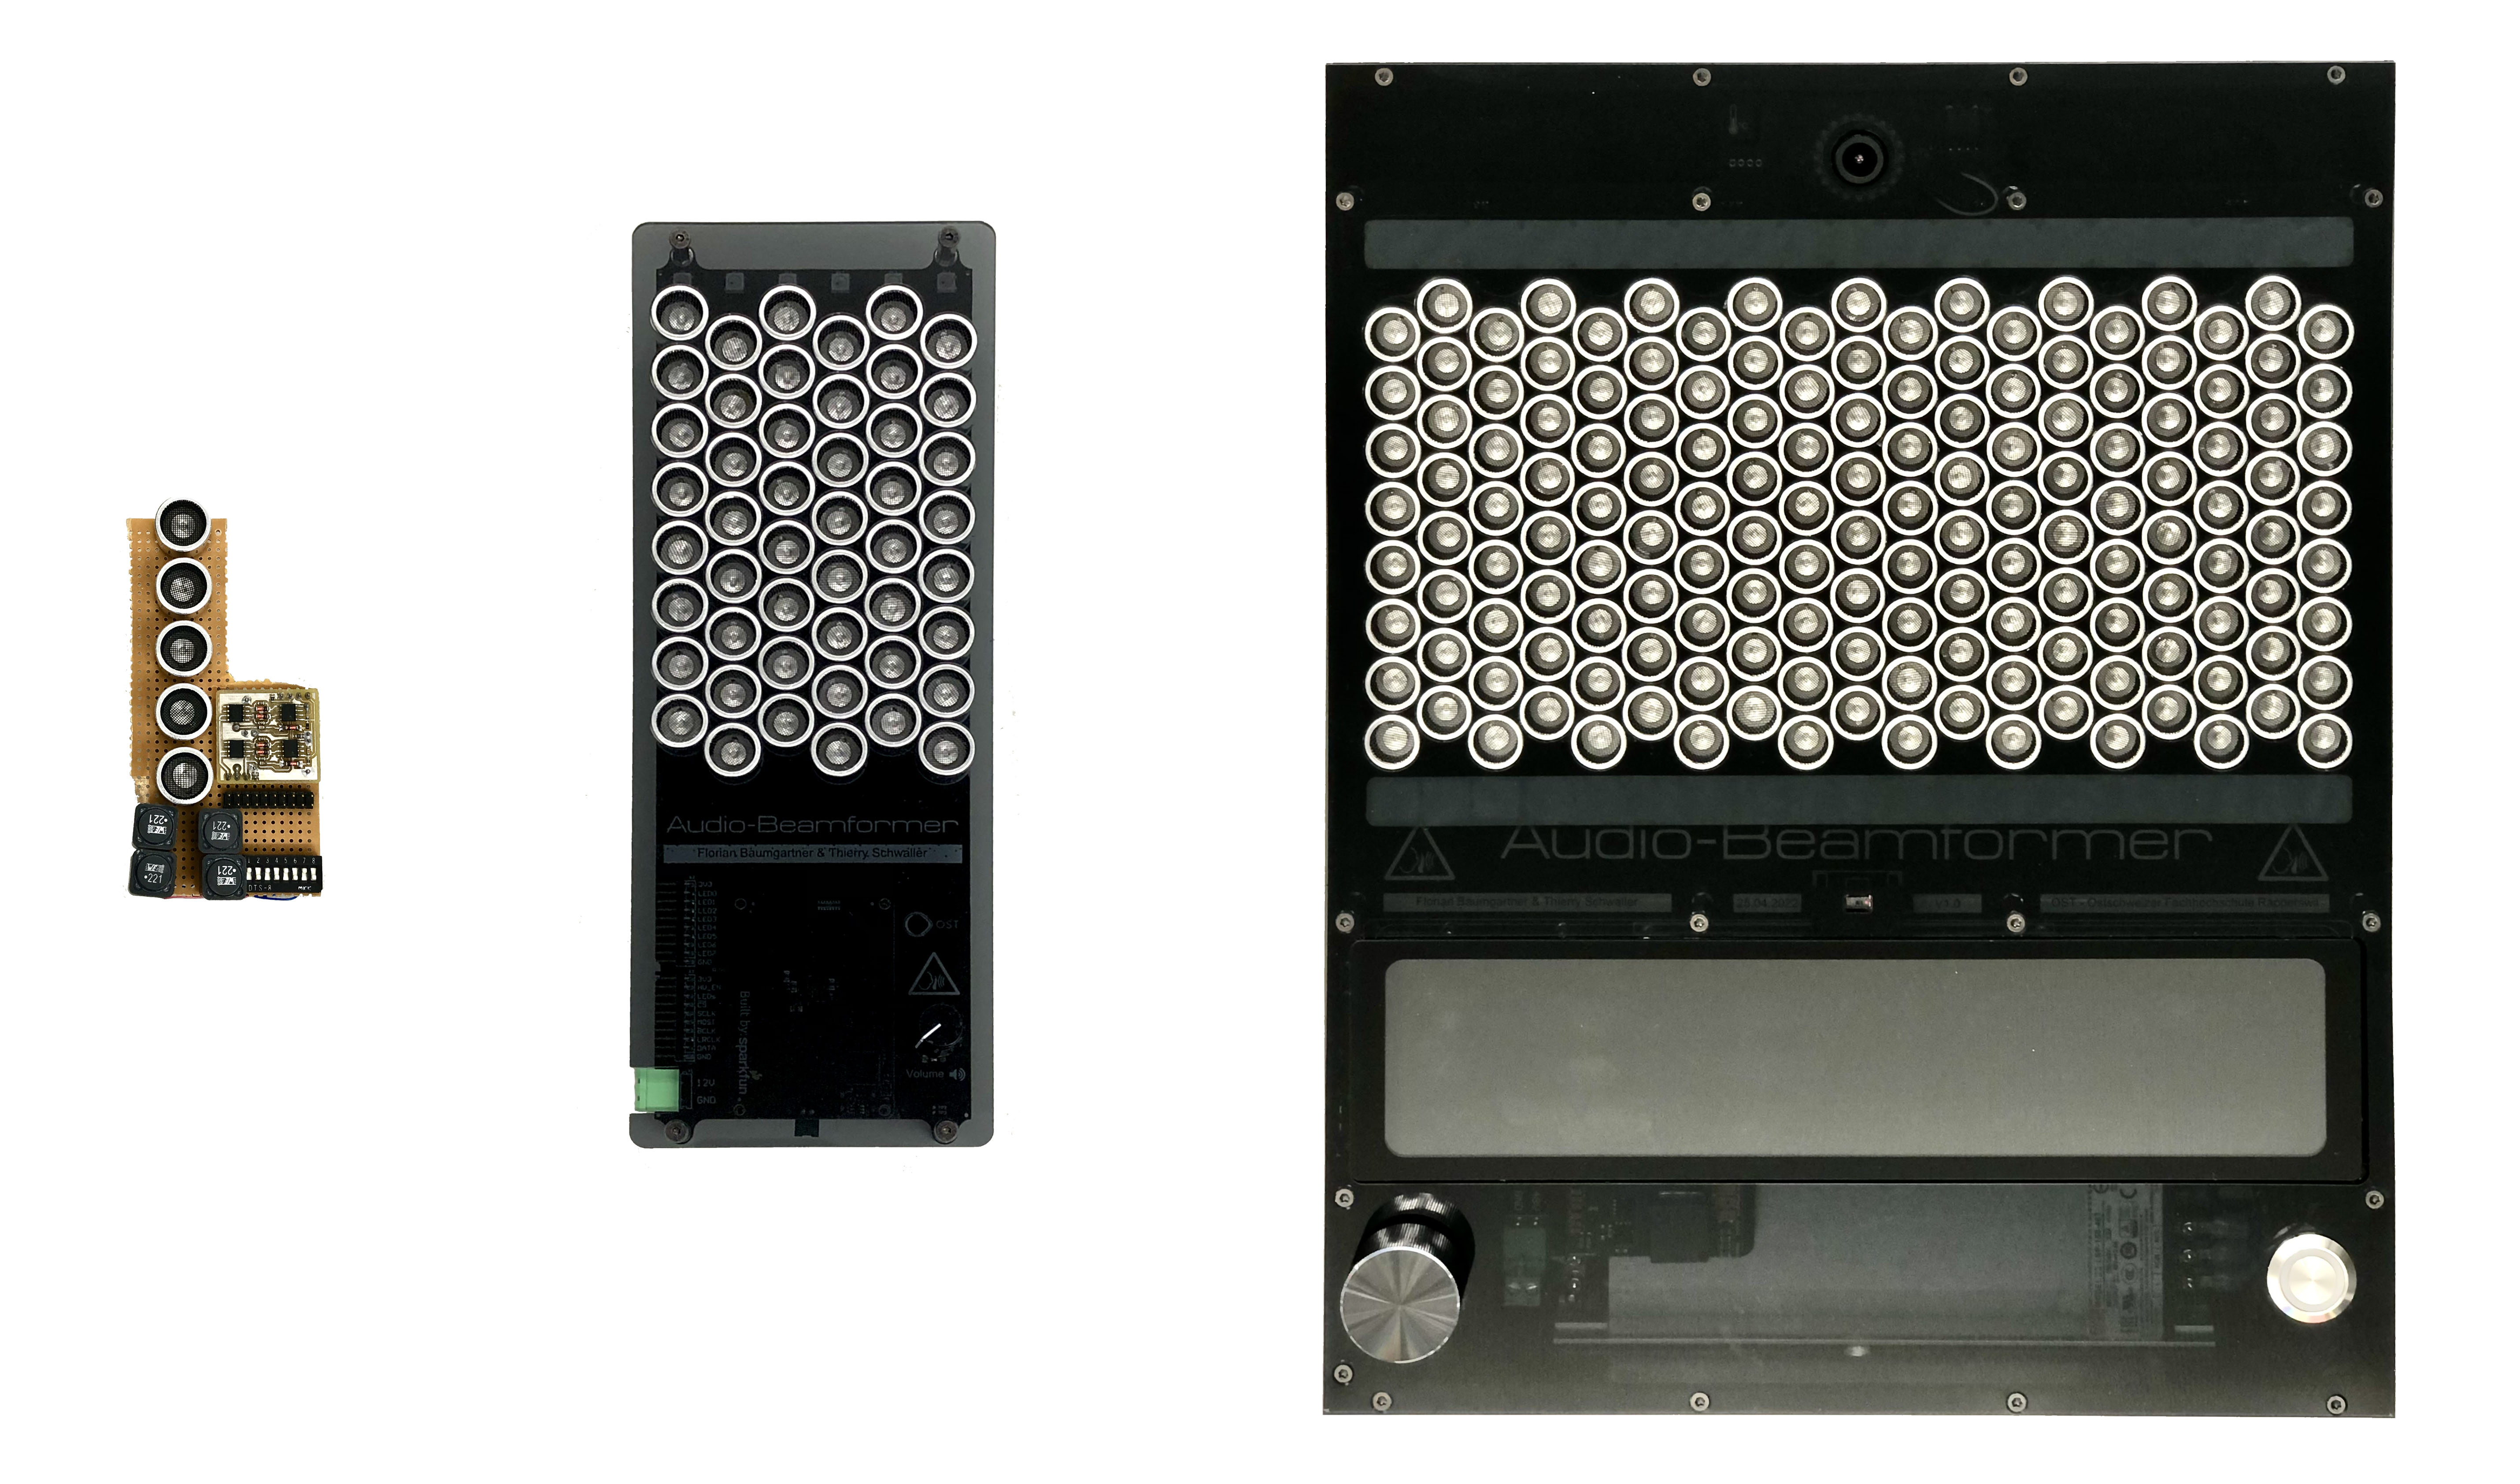
\includegraphics[width=\textwidth]{images/1_Introduction/Approach.jpg}
	\vspace{-0.4cm}
    \caption{Hardware Prototype Revisions}
    \label{fig:prototype_revisions}
\end{figure}


\section{Open Source}
From the beginning, it was decided that everything about the project would be released under an open source license. Both of us are huge supporters of open source and believe it will be the future of engineering. Building upon existing libraries and code under open source licenses, allows us to accelerate the design process. Sometimes open source is considered an act of charity, but in our case, the benefits of using it outweigh any closed source processes. All documents and files for this project can be found on our GitHub page. A short description of all the repositories can be found in the Appendix \ref{Data Archive}.
